% =====================================================================
%  6. RISK MANAGEMENT
% =====================================================================
\section{Risk Management}\label{sec:risk}

% Risk rating colours (used in the matrix and the register)
\definecolor{risklow}{HTML}{BBF7D0}
\definecolor{riskmed}{HTML}{FDE68A}
\definecolor{riskhigh}{HTML}{FDBA74}
\definecolor{riskcrit}{HTML}{FCA5A5}
\newcommand{\rlow}[1]{\cellcolor{risklow}Low (#1)}
\newcommand{\rmed}[1]{\cellcolor{riskmed}Medium (#1)}
\newcommand{\rhigh}[1]{\cellcolor{riskhigh}High (#1)}
\newcommand{\rcrit}[1]{\cellcolor{riskcrit}Critical (#1)}

A risk is an uncertain event or condition that, if it occurs, affects one or more project objectives \parencite{pmi2021pmbok}. Because \projectname{} depends on external parties (the dataset authors, ethics requirements and study participants) and has three fixed assessment deadlines, risks are managed actively from the first week rather than only when problems arise.

\subsection{Risk Management Approach}\label{sec:risk-approach}

Risks are managed through a continuous cycle of five steps:

\begin{enumerate}[nosep]
  \item \textbf{Identify.} Initial risks were identified at project kick-off by reviewing the requirements, the assumptions and constraints (Section~\ref{sec:assumptions}), the schedule's critical path (Section~\ref{sec:schedule}) and the PRISMO paper's stated limitations. New risks can be raised by any member at any time.
  \item \textbf{Assess.} Each risk is rated for likelihood and impact on a five-point scale (Table~\ref{tab:risk-scales}). Its score is likelihood $\times$ impact, which places it in the risk assessment matrix (Figure~\ref{fig:risk-matrix}).
  \item \textbf{Plan responses.} Each risk is given an owner and a response strategy: \emph{avoid} (remove the cause), \emph{mitigate} (reduce likelihood or impact), \emph{transfer} (shift ownership to a party better placed to manage it) or \emph{accept} (take no action now but monitor it). Most risks also have a contingency plan that is put into action if a defined \emph{trigger} occurs.
  \item \textbf{Monitor.} The risk register is reviewed at every weekly team meeting. Owners report on their risks' status and triggers, scores are updated, and closed risks are marked as such.
  \item \textbf{Escalate.} High and Critical risks are reported to the tutor at the next consultation. Using the contingency reserve (70 hours; Section~\ref{sec:wbs-dictionary}) to respond to a risk requires the Project Manager's approval. Any response that changes scope, schedule or deliverables goes through change control (Section~\ref{sec:change-control}).
\end{enumerate}

\begin{table}[htbp]
\centering
\caption{Likelihood and impact rating scales}
\label{tab:risk-scales}
\begin{tabularx}{\textwidth}{@{}c >{\raggedright\arraybackslash}p{0.3\textwidth} >{\raggedright\arraybackslash}X@{}}
  \toprule
  \textbf{Rating} & \textbf{Likelihood} & \textbf{Impact} \\
  \midrule
  1 & Rare (less than 10\%) & Negligible: under one day of delay; no effect on deliverables \\
  2 & Unlikely (10--30\%) & Minor: one to two days of delay or minor rework \\
  3 & Possible (30--50\%) & Moderate: three to five days of delay, or a Should requirement lost \\
  4 & Likely (50--80\%) & Major: more than a week of delay, or a Must requirement or assessment quality at risk \\
  5 & Almost certain (over 80\%) & Severe: an assessment deadline is missed or the project cannot be completed \\
  \bottomrule
\end{tabularx}
\par\smallskip
{\footnotesize \textbf{Risk score} = likelihood $\times$ impact. \quad
\colorbox{risklow}{Low: 1--4} \enspace
\colorbox{riskmed}{Medium: 5--9} \enspace
\colorbox{riskhigh}{High: 10--16} \enspace
\colorbox{riskcrit}{Critical: 20--25}}
\end{table}

\subsection{Risk Assessment Matrix}\label{sec:risk-matrix}

Figure~\ref{fig:risk-matrix} shows where each identified risk falls by likelihood and impact. No risk is currently rated Critical. Five risks are rated High (R1, R2, R3, R5 and R8). They relate to the dataset, ethics approval, the tight Assignment~2 timeline and team availability, and each has an active response plan.

\begin{figure}[htbp]
\centering
% =====================================================================
%  Risk assessment matrix -- generated; colours defined in sections/06-risk.tex
% =====================================================================
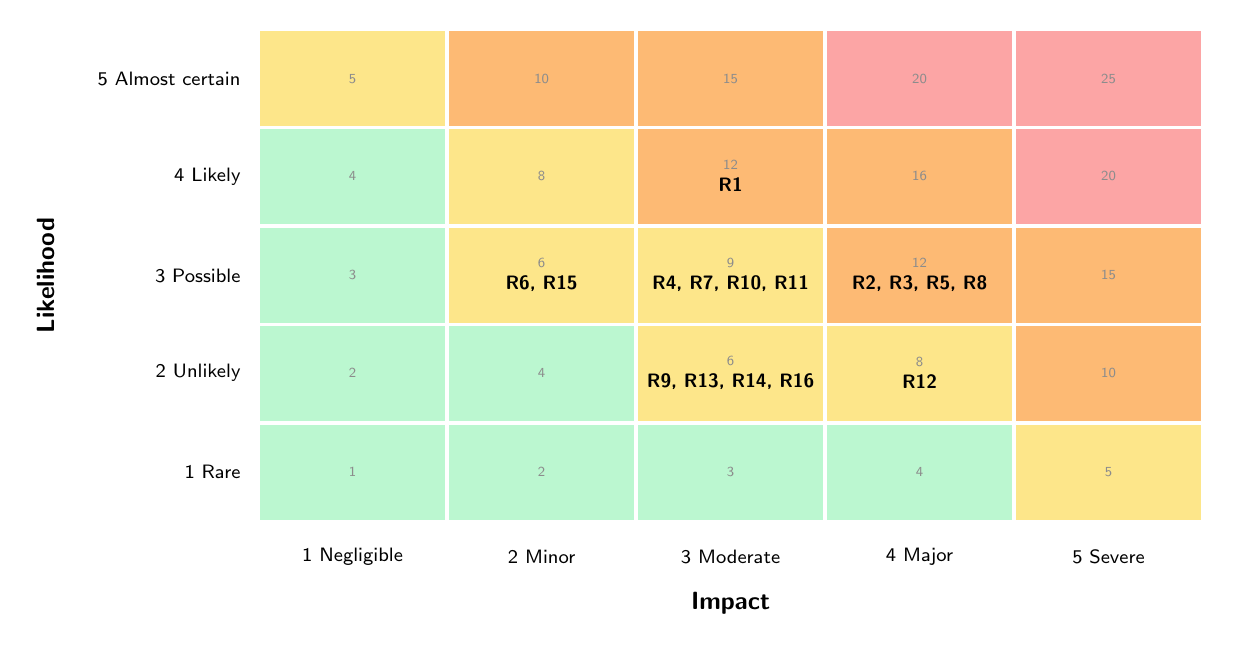
\begin{tikzpicture}[cell/.style={draw=white, line width=1.2pt, minimum width=2.4cm, minimum height=1.25cm,
      align=center, font=\scriptsize\sffamily, text width=2.2cm, inner sep=1pt}]
  \node[cell, fill=risklow] at (1.20,0.62) {{\color{black!45}\tiny 1}};
  \node[cell, fill=risklow] at (3.60,0.62) {{\color{black!45}\tiny 2}};
  \node[cell, fill=risklow] at (6.00,0.62) {{\color{black!45}\tiny 3}};
  \node[cell, fill=risklow] at (8.40,0.62) {{\color{black!45}\tiny 4}};
  \node[cell, fill=riskmed] at (10.80,0.62) {{\color{black!45}\tiny 5}};
  \node[cell, fill=risklow] at (1.20,1.88) {{\color{black!45}\tiny 2}};
  \node[cell, fill=risklow] at (3.60,1.88) {{\color{black!45}\tiny 4}};
  \node[cell, fill=riskmed] at (6.00,1.88) {{\color{black!45}\tiny 6}\\\textbf{R9, R13, R14, R16}};
  \node[cell, fill=riskmed] at (8.40,1.88) {{\color{black!45}\tiny 8}\\\textbf{R12}};
  \node[cell, fill=riskhigh] at (10.80,1.88) {{\color{black!45}\tiny 10}};
  \node[cell, fill=risklow] at (1.20,3.12) {{\color{black!45}\tiny 3}};
  \node[cell, fill=riskmed] at (3.60,3.12) {{\color{black!45}\tiny 6}\\\textbf{R6, R15}};
  \node[cell, fill=riskmed] at (6.00,3.12) {{\color{black!45}\tiny 9}\\\textbf{R4, R7, R10, R11}};
  \node[cell, fill=riskhigh] at (8.40,3.12) {{\color{black!45}\tiny 12}\\\textbf{R2, R3, R5, R8}};
  \node[cell, fill=riskhigh] at (10.80,3.12) {{\color{black!45}\tiny 15}};
  \node[cell, fill=risklow] at (1.20,4.38) {{\color{black!45}\tiny 4}};
  \node[cell, fill=riskmed] at (3.60,4.38) {{\color{black!45}\tiny 8}};
  \node[cell, fill=riskhigh] at (6.00,4.38) {{\color{black!45}\tiny 12}\\\textbf{R1}};
  \node[cell, fill=riskhigh] at (8.40,4.38) {{\color{black!45}\tiny 16}};
  \node[cell, fill=riskcrit] at (10.80,4.38) {{\color{black!45}\tiny 20}};
  \node[cell, fill=riskmed] at (1.20,5.62) {{\color{black!45}\tiny 5}};
  \node[cell, fill=riskhigh] at (3.60,5.62) {{\color{black!45}\tiny 10}};
  \node[cell, fill=riskhigh] at (6.00,5.62) {{\color{black!45}\tiny 15}};
  \node[cell, fill=riskcrit] at (8.40,5.62) {{\color{black!45}\tiny 20}};
  \node[cell, fill=riskcrit] at (10.80,5.62) {{\color{black!45}\tiny 25}};
  \node[font=\scriptsize\sffamily, align=center] at (1.20,-0.45) {1~Negligible};
  \node[font=\scriptsize\sffamily, align=center] at (3.60,-0.45) {2~Minor};
  \node[font=\scriptsize\sffamily, align=center] at (6.00,-0.45) {3~Moderate};
  \node[font=\scriptsize\sffamily, align=center] at (8.40,-0.45) {4~Major};
  \node[font=\scriptsize\sffamily, align=center] at (10.80,-0.45) {5~Severe};
  \node[font=\scriptsize\sffamily, anchor=east] at (-0.1,0.62) {1~Rare};
  \node[font=\scriptsize\sffamily, anchor=east] at (-0.1,1.88) {2~Unlikely};
  \node[font=\scriptsize\sffamily, anchor=east] at (-0.1,3.12) {3~Possible};
  \node[font=\scriptsize\sffamily, anchor=east] at (-0.1,4.38) {4~Likely};
  \node[font=\scriptsize\sffamily, anchor=east] at (-0.1,5.62) {5~Almost certain};
  \node[font=\small\sffamily\bfseries] at (6.00,-1.05) {Impact};
  \node[font=\small\sffamily\bfseries, rotate=90] at (-2.7,3.12) {Likelihood};
\end{tikzpicture}

\caption{Risk assessment matrix showing the current rating of each risk}
\label{fig:risk-matrix}
\end{figure}

\subsection{Risk Register}\label{sec:risk-register}

Table~\ref{tab:risk-register} lists every identified risk with its cause and effect, category, rating and owner. Owners are identified by the initials used in Section~\ref{sec:wbs-dictionary}.

{\renewcommand{\arraystretch}{1.2}\small
\begin{longtable}{@{}l >{\raggedright\arraybackslash}p{0.45\textwidth} >{\raggedright\arraybackslash}p{0.12\textwidth} c c l l@{}}
  \caption{Risk register}\label{tab:risk-register} \\
  \toprule
  \textbf{ID} & \textbf{Risk (cause, event and effect)} & \textbf{Category} & \textbf{L} & \textbf{I} & \textbf{Rating} & \textbf{Owner} \\
  \midrule
  \endfirsthead
  \multicolumn{7}{@{}l}{\small\itshape Table~\thetable{} continued} \\
  \toprule
  \textbf{ID} & \textbf{Risk (cause, event and effect)} & \textbf{Category} & \textbf{L} & \textbf{I} & \textbf{Rating} & \textbf{Owner} \\
  \midrule
  \endhead
  \midrule
  \multicolumn{7}{@{}r}{\small\itshape Continued on next page} \\
  \endfoot
  \bottomrule
  \multicolumn{7}{@{}l}{\footnotesize\parbox{\textwidth}{\vspace{0.3em}L = likelihood; I = impact (Table~\ref{tab:risk-scales}). Owners: TKN = \memberOne; NMV = \memberTwo; HDN = \memberThree; NKNT = \memberFour.}} \\
  \endlastfoot
  R1 & The PRISMO dataset is released only on request, so the authors may not reply, or may refuse access, by the decision date (12 Oct), forcing a switch to a fallback dataset and preventing a direct comparison with PRISMO. & Data & 4 & 3 & \rhigh{12} & TKN \\
  R2 & If a fallback dataset is used, computing PRISMO-equivalent features from raw account and tweet data takes longer than planned, delaying feature selection and Assignment~2. & Data / Schedule & 3 & 4 & \rhigh{12} & TKN \\
  R3 & The user study may require ethics approval that cannot be obtained before the study is scheduled (23--30 Nov), so RQ2--RQ5 cannot be answered with external participants. & Ethics / Scope & 3 & 4 & \rhigh{12} & TKN \\
  R4 & Too few participants volunteer for the user study because of competing assessments, weakening the evidence for RQ2--RQ5. & Evaluation & 3 & 3 & \rmed{9} & NMV \\
  R5 & The GA, PSO and SA experiments take longer to implement or run than planned, because each fitness evaluation trains a classifier, so the Assignment~2 critical path overruns. & Technical / Schedule & 3 & 4 & \rhigh{12} & NKNT \\
  R6 & PRISMO's unreported parameters and ambiguous Layer~2 description lead to results that differ noticeably from the paper, making RQ1 harder to answer. & Technical & 3 & 2 & \rmed{6} & NMV \\
  R7 & The selected model does not reach the target macro F1-score of 0.85 or a spammer detection rate above 72.4\% (NFR1), for example because of class imbalance. & Technical & 3 & 3 & \rmed{9} & NKNT \\
  R8 & Members cannot sustain about 12 hours per week because of other units' assessments, work or illness, reducing capacity below the planned 386 hours. & Resource & 3 & 4 & \rhigh{12} & TKN \\
  R9 & Application work is concentrated in Stage~3 (Weeks 5--8), when the front end, back end, charts and decision-support features are all being built, which could overload the members leading them. & Resource & 2 & 3 & \rmed{6} & TKN \\
  R10 & Differences between the experiment environment and the FastAPI back end (library versions, model serialisation, pre-processing) cause integration failures or inconsistent predictions. & Technical & 3 & 3 & \rmed{9} & HDN \\
  R11 & Scope creep, such as adding live data collection, extra models or features beyond the plan, diverts effort from core requirements. & Scope & 3 & 3 & \rmed{9} & TKN \\
  R12 & Code, data or documents are lost or overwritten through conflicting edits or a device failure. & Technical & 2 & 4 & \rmed{8} & HDN \\
  R13 & The PRISMO dataset's terms of use may not allow the processed data to be included in the Assignment~2 ZIP file, which requires processed datasets. & Data / Legal & 2 & 3 & \rmed{6} & TKN \\
  R14 & Plain-language explanations are inaccurate or misleading (e.g.\ wrong reference values), causing users to misjudge accounts and invalidating RQ3 and RQ4. & Quality & 2 & 3 & \rmed{6} & NKNT \\
  R15 & Members are unfamiliar with some technologies (React, FastAPI, charting libraries, SHAP, optimisation libraries), slowing development. & Technical & 3 & 2 & \rmed{6} & HDN \\
  R16 & Poor communication or uneven contribution causes duplicated work, missed hand-overs or team conflict. & Team & 2 & 3 & \rmed{6} & TKN \\
\end{longtable}
}

\subsection{Risk Response Plan}\label{sec:risk-plan}

Table~\ref{tab:risk-response} sets out the response strategy, preventive actions, contingency plan and trigger for each risk. Preventive actions are carried out as part of normal project work. Contingency plans are put into action by the risk owner as soon as the trigger occurs, and reported at the next team meeting.

{\renewcommand{\arraystretch}{1.2}\small
\begin{longtable}{@{}l >{\raggedright\arraybackslash}p{0.09\textwidth} >{\raggedright\arraybackslash}p{0.31\textwidth} >{\raggedright\arraybackslash}p{0.28\textwidth} >{\raggedright\arraybackslash}p{0.14\textwidth}@{}}
  \caption{Risk response plan}\label{tab:risk-response} \\
  \toprule
  \textbf{ID} & \textbf{Strategy} & \textbf{Preventive Actions} & \textbf{Contingency Plan} & \textbf{Trigger} \\
  \midrule
  \endfirsthead
  \multicolumn{5}{@{}l}{\small\itshape Table~\thetable{} continued} \\
  \toprule
  \textbf{ID} & \textbf{Strategy} & \textbf{Preventive Actions} & \textbf{Contingency Plan} & \textbf{Trigger} \\
  \midrule
  \endhead
  \midrule
  \multicolumn{5}{@{}r}{\small\itshape Continued on next page} \\
  \endfoot
  \bottomrule
  \endlastfoot
  R1 & Mitigate & Request the dataset on 5 Oct, clearly explaining the academic purpose; download Cresci-2017 in Week~1; write feature-computation scripts in parallel. & Switch to Cresci-2017 at M5; compare with PRISMO's reported ranges and method rather than its exact figures. & No reply by Fri 9 Oct, or access refused \\
  R2 & Mitigate & Prioritise the PRISMO features that can be computed directly from raw data; reuse the definitions of \textcite{benevenuto2010detecting}; split the computation across two members. & Use contingency hours; reduce to the computable subset of features and document the difference. & Feature preparation not finished by Tue 20 Oct \\
  R3 & Mitigate & Ask the tutor about ethics requirements by 9 Oct (M3); design a low-risk, anonymous study; prepare consent and study materials early. & Replace the external study with an internal heuristic evaluation and cognitive walkthrough with the team and tutor; report RQ2--RQ5 as exploratory. & Approval required and not granted by Fri 20 Nov \\
  R4 & Mitigate & Recruit from Week~6; keep sessions to about 20 minutes; offer online sessions; arrange reciprocal testing with other groups. & Run with fewer participants and report the results as exploratory, supported by qualitative feedback. & Fewer than 6 participants confirmed by Mon 23 Nov \\
  R5 & Mitigate & Implement and test the algorithms on sample data in Week~2; use a cheaper fitness evaluation (e.g.\ 3-fold cross-validation and moderate population sizes); run experiments in parallel on several laptops. & Reduce iterations and the number of runs; document the reduced settings in the Assignment~2 report. & Any algorithm not producing a subset by Sun 25 Oct \\
  R6 & Accept & Document every parameter and interpretation (NFR9); compare selected features with the subsets listed in the paper. & Report the differences and their likely causes; a documented difference is still a valid answer to RQ1. & Results outside the paper's reported ranges \\
  R7 & Mitigate & Apply class weighting and decision-threshold tuning; consider the optional gradient-boosting model. & Report the achieved performance honestly; adjust the target through change control if it proves unrealistic. & Best macro F1 below 0.85 at M8 \\
  R8 & Mitigate & Hold the 15\% contingency reserve; make workload visible on the task board; share upcoming deadlines from other units at weekly meetings. & Re-plan the following week's tasks; defer Should and Could requirements; scale down the user study if needed. & A member misses planned hours for two consecutive weeks \\
  R9 & Mitigate & Agree the API contract early (5.1) so that components can be built in parallel; spread application tasks across members (charts by NMV, decision support by NKNT); the Project Manager, who has full-stack skills, and other members support front-end and back-end tasks as needed. & Reassign tasks at the weekly meeting; the Project Manager or another member takes over specific components. & Any application package more than three days behind schedule \\
  R10 & Mitigate & Package pre-processing as a reusable pipeline (2.3); pin library versions in a shared requirements file; connect a mock model early; run an integration test at M8. & Re-export the model in the back end's environment; wrap the pipeline behind a single prediction function. & Failed integration test, or predictions differ between notebook and API \\
  R11 & Avoid & Enforce the core and stretch tiers; all new requests go through change control; code freeze at M12. & Reject or defer the change; record it in the change log. & Work starts on an item not in the WBS \\
  R12 & Mitigate & Use GitHub with feature branches and reviewed pull requests; store datasets and documents in a shared cloud folder; Overleaf for this document. & Restore from the repository or cloud backup. & Any lost or overwritten work \\
  R13 & Transfer & Ask the dataset authors, in the access request, whether processed data may be included in a private assessment submission. & Submit only derived features or a sample with preparation scripts, or use the public fallback dataset. & Terms prohibit redistribution \\
  R14 & Mitigate & Generate explanations directly from SHAP values; test the explanation text against known cases; have NMV review the reference values. & Correct the explanation logic and re-run the affected checks before the user study. & Any explanation that contradicts the model's actual feature contributions \\
  R15 & Mitigate & HDN and TKN run a short onboarding session on React and FastAPI early in Week~5, as application work begins; use shared project templates; pair programming for first tasks. & Pair the member with an experienced teammate; simplify the component if needed. & A task takes more than twice its estimate \\
  R16 & Avoid & Weekly meetings with minutes; a shared task board; a team charter agreed at kick-off; contributions visible through GitHub. & The Project Manager addresses issues directly; escalate to the tutor if unresolved. & Missed hand-over or unresolved conflict \\
\end{longtable}
}
